% v2-acmsmall-sample.tex, dated March 6 2012
% This is a sample file for ACM small trim journals
%
% Compilation using 'acmsmall.cls' - version 1.3 (March 2012), Aptara Inc.
% (c) 2010 Association for Computing Machinery (ACM)
%
% Questions/Suggestions/Feedback should be addressed to => "acmtexsupport@aptaracorp.com".
% Users can also go through the FAQs available on the journal's submission webpage.
%
% Steps to compile: latex, bibtex, latex latex
%
% For tracking purposes => this is v1.3 - March 2012

\documentclass[prodmode,acmtecs]{acmsmall} % Aptara syntax

% Package to generate and customize Algorithm as per ACM style
\usepackage[ruled]{algorithm2e}
\renewcommand{\algorithmcfname}{ALGORITHM}
\SetAlFnt{\small}
\SetAlCapFnt{\small}
\SetAlCapNameFnt{\small}
\SetAlCapHSkip{0pt}
\IncMargin{-\parindent}

\usepackage{cite}
\usepackage{amsmath,amssymb,amsfonts}
\usepackage{algorithmic}
\usepackage{graphicx}
\usepackage{textcomp}
\usepackage{xcolor}
\usepackage{float}
\usepackage{amsmath}
%\usepackage{subcaption}
%\usepackage{subfig}
\usepackage{subfigure}
\DeclareMathOperator*{\argmax}{arg\,max}
\DeclareMathOperator*{\argmin}{arg\,min}
\usepackage{graphicx}
\usepackage{svg}

%\usepackage{subcaption}

% Metadata Information
%\acmVolume{9}
%\acmNumber{4}
%\acmArticle{}
%\acmYear{2010}
%\acmMonth{3}

% Document starts
\begin{document}

% Page heads
%\markboth{G. Zhou et al.}{A Multifrequency MAC Specially Designed for WSN Applications}

% Title portion
\title{Comparison of Outlier Detection between Statistical Method and Undercomplete Autoencoder}
\author{Muhammad Ayaz Hussain
\affil{University of}
Saif ur Rahman
\affil{University of}
Christian Klaus 
\affil{University of}
Ioannis Iossifidis
\affil{University of}
}
% NOTE! Affiliations placed here should be for the institution where the
%       BULK of the research was done. If the author has gone to a new
%       institution, before publication, the (above) affiliation should NOT be changed.
%       The authors 'current' address may be given in the "Author's addresses:" block (below).
%       So for example, Mr. Abdelzaher, the bulk of the research was done at UIUC, and he is
%       currently affiliated with NASA.

\begin{abstract}
This paper is concerned about the analysis of power consumption data and the comparison of the performance between statistical method and undercomplete autoencoder in the determination of outliers in that given dataset. Firstly, the raw data was analyzed and a feature vector was constructed. Secondly, Tukey's test was implemented on this feature vector to determine the outliers. Finally, an undercomplete autoencoder was also used to detect outliers and the efficiency of both methods (statistical method and undercomplete autoencoder) were compared.
 %As power consumption varies over time, therefore the labeled data created by that becomes obsolete overtimes. Therefore, supervised learning is not a viable method in the prediction of energy consumption over a long period of time.
\end{abstract}

%\category{C.2.2}{Computer-Communication Networks}{Network Protocols}

%\terms{Design, Algorithms, Performance}

%\keywords{Wireless sensor networks, media access control,
%multi-channel, radio interference, time synchronization}

%\acmformat{Gang Zhou, Yafeng Wu, Ting Yan, Tian He, Chengdu Huang, John A. Stankovic,
%and Tarek F. Abdelzaher, 2010. A multifrequency MAC specially
%designed for  wireless sensor network applications.}
% At a minimum you need to supply the author names, year and a title.
% IMPORTANT:
% Full first names whenever they are known, surname last, followed by a period.
% In the case of two authors, 'and' is placed between them.
% In the case of three or more authors, the serial comma is used, that is, all author names
% except the last one but including the penultimate author's name are followed by a comma,
% and then 'and' is placed before the final author's name.
% If only first and middle initials are known, then each initial
% is followed by a period and they are separated by a space.
% The remaining information (journal title, volume, article number, date, etc.) is 'auto-generated'.

%\begin{bottomstuff}
%This work is supported by the National Science Foundation, under
%grant CNS-0435060, grant CCR-0325197 and grant EN-CS-0329609.

%Author's addresses: G. Zhou, Computer Science Department,
%College of William and Mary; Y. Wu  {and} J. A. Stankovic,
%Computer Science Department, University of Virginia; T. Yan,
%Eaton Innovation Center; T. He, Computer Science Department,
%University of Minnesota; C. Huang, Google; T. F. Abdelzaher,
%(Current address) NASA Ames Research Center, Moffett Field, California 94035.
%\end{bottomstuff}

\maketitle


\section{Introduction}

In modern days, the amount of energy consumption is becoming a more serious issue as several companies and industries are addressing this issue in order to contain their expenses as unexpected variations can incur additional operational costs to their facilities. These fluctuations in electricity consumption can arise from various factors such as excessive use of heavy equipment like electric heaters in winters, room coolers during the summers etc. In order to detect and classify unusual amount of power consumption, outlier detection algorithm is designed and implemented on the provided data and compared its classification efficiency against a semi-supervised autoencoder.
Presently, it is very difficult to predict the energy consumption anomalies precisely, since there are many factors influencing the energy usage, such as weather condition \cite{WANG2012152},  occupancy \cite{PAN2007651} and operation of appliances \cite{7260948,ROYAPOOR2015109}
% quote
%\begin{quote}
%``For these applications, sensor devices are incorporated into human
%cloths [Natarajan 2001,Zhou 2006,Bahl 2002,Adya 2001] for monitoring
%health related information like EKG readings, fall detection, and voice recognition".
%\end{quote}

% itemize
%\begin{itemize}
%\item To the best of our knowledge, the MMSN protocol is the first
%multifrequency MAC protocol especially designed for WSNs, in which
%each device is equipped with a single radio transceiver and
%the MAC layer packet size is very small.
%\item Instead of using pairwise RTS/CTS frequency negotiation
%[Adya 2001,Culler 2001; Tzamaloukas 2001; Zhou 2006],
%we propose lightweight frequency assignments, which are good choices
%for many deployed comparatively static WSNs.
%\item We develop new toggle transmission and snooping techniques to
%enable a single radio transceiver in a sensor device to achieve
%scalable performance, avoiding the nonscalable ``one
%control channel + multiple data channels'' design [Natarajan 2001].
%\end{itemize}

% Head 1

\section{Related Works}
There is a sizable literature regarding semi-supervised learning methods on big data, with some relating to power consumption such as, 
\cite{Bhattacharjee:2018:TFS:3196494.3196551} which also performed semi-supervised analysis to determine and counter data falsifications in power consumption which can be considered as anomalous power consumption. Since data falsification can range from individual customers tampering with the meter for electricity theft to certain groups orchestrating an attack against a rival company in a systematic manner compromising several meters, as their goals can be more complex than just electricity theft. For that, they proposed, a novel metric based on harmonic to the arithmetic mean ratios of daily power consumption. The ratios between harmonic and arithmetic mean remain highly stable over time as compared to just arithmetic mean. During various attacks, there is asymmetric growth(or decay) rates harmonic mean as compared to symmetric growth(or decay) rates of the arithmetic mean, which can help to infer the presence and type of falsification precisely. Their data consisted of real power consumption of 700 houses from Texas and 5000 houses from Ireland that belong to residential customers. One of the most important aspect of this work is that, it enables the quick identification of around or less than 10 days of monitoring, which is quite efficient as compared to pattern-based energy theft detector (CPBETD) which takes around 1 year, autoregressive moving average (ARMA) which took 1 month, or Entropy based method which also took 1 month.
 
%Our statistical approach also deals with the analysis of power consumption data to find any short term anomalous readings, which performs quite well as more than 95\% anomalies were detected successfully using Tukey test (which uses arithmetic means and 1st and 3rd quartiles which is discussed in \ref{sec:level2}) 

As far as the use of autoencoder for classification is concerned, those have been used in previous works for classification tasks such as \cite{FAN20181123} which used autoencoder based unsupervised anomaly detection method on a building energy data on a single facility which was in detail as 113 variables were considered which were generally classified into 4 distinct classes which are,  (1) time variables (i.e.,
Month, Day, Hour, Minute and Day type); (2) outdoor variables (e.g., outdoor dry-bulb temperature and relative humidity); (3) operating parameters of the chiller plant (e.g., the temperatures and flow-rates of chilled
water and condenser water); (4) energy variables (e.g., the total building
cooling load and electricity consumption of the chiller plant).The
highest classification accuracy is achieved using the high-level features
generated by the 1D convolutional autoencoder trained without conditional information and using a 10\% masking noise level. In general,
convolutional autoencoders have slightly better performance than the
feed-forward fully connected autoencoders.  Similar to other machine learning problems, the accuracy of classification depends upon the quality of dataset. Since they used a vast number of variables in their feature vector, therefore, unsupervised learning was possible. 


Semi-supervised learning using Softmax classifier with  sparse autoencoder for classification of water quality is done by \cite{article123}. Their dataset consisted of 60 unbalanced classification records, 100 training samples are generated for each water quality assesment grade. Their feature vector consisted of 14 representative features of water quality which were chemical oxygen demand (COD), dissolved oxygen
(DO), total phosphorus (TP), 5-day biochemical oxygen demand (BOD5), NH3-N, NO3-
N, oil, chlorophyll, PH, electrical conductivity (EC), turbidity, CL, total coliform (TColi)
and temperature (T). They used 500 labeled training samples and 7,932 unlabeled records in all. Their proposed method method showed 98.8\% accuracy which was greater as compared to other supervised algorithms such as Softmax classifiers, BP-NN, RBF-NN and SVM.  
%Previous studies in data-driven building energy consumption prediction have utilized several methods such as engineering methods \cite{ZHAO20123586}, statistical methods \cite{5301031}, Artificial Neural Networks (ANN) \cite{EKICI2009356,KUSIAK2010925}, Support Vector Machines (SVM) \cite{LI20092249}, fuzzy logic and grey model techniques \cite{GUO20111273}, decision trees \cite{TSO20071761} etc. 

%Also there have been some studies which compared the effectiveness of different algorithms in energy consumption prediction by comparing the results of two or more algorithms on a similar dataset. For example, \cite{LI20092249} compared SVM and Back Propagation Neural Network (BPNN) to predict hourly cooling load in
%a building ; %Borges et al. \cite{bb11} compared SVM and Autoregressive (AR) Model;%
%\cite{5196994}  compared LS-SVM and BPNN for building cooling load forecasting; \cite{6606376}  compared Support Vector Regression (SVR) and ANN for lighting consumption for a building; \cite{5984356,6059103} compared AR Model, ANN, autoregressive integrated moving average (ARIMA), and Bayesian Network on a university campus for short term load forecasting by incorporating energy information as well as metrological data; \cite{PLATON201510}  compared ANN and Case based Reasoning (CBR) for the prediction of hourly electricity consumption of an institutional building; \cite{doi:10.1061/9780784413616.208} compared SVM and MLR to forecast energy consumption on a multi-family residential building;  \cite{HOU20061033} compared ARIMA and ANN (need to download paper);  \cite{FAN20141}  compared MLR, ARIMA, SVM, RF, MLP, BT, MARS, and kNN on a high rise commercial building ; \cite{CHOU2014437} emphasized on building geometry in their dataset while comparing ANN, SVM, CART, CHAID, and GLR ; \cite{EDWARDS2012591}  compared MLR, FFNN, SVM, LS-SVM, HME-FFNN, and FCM-FFNN in predicting residential electricity consumption; \cite{LI200990,5557576} compared SVM, BPNN, Radial Basis Function Neural Network (RBFNN), and General Regression Neural Network (GRNN) on multiple residential buildings; Dagnely et al. \cite{Dagnely:2015:PHE:2964895.2964903} compared Ordinary Least Squared (OLS) Regression and SVR for the prediction of hourly energy consumption by taking temporal predictors such as occupancy, working hours and days of the week as well as metrological predictors such as ambient temperature and irradiance for a building;  \cite{MASSANA2015322} compared MLR, MLP, and SVR for Short-term load forecasting in a non-residential building. A hybrid neural net ARIMA have been used by Chou et al.\cite{CHOU2014437} to detect anomalies in the power consumption in an office space. In another paper, Capozolli et al. \cite{CAPOZZOLI20154324} used Classification and Regression Tree (CART), K-Mean clustering, Artificial neural networks and basic ensembling method (ANN BEM) and Outlier Detection methods such as Generalized Extreme Studentized Deviation (GESD) and Peak detection method on a building cluster. Whereas, \cite{en6042110} compared SVM and Autoregressive (AR) Model on the energy consumption on a couple of university campuses for a load forecasting. 






%As far as the use of autoencoder for classification is concerned, those have been used in previous works for classification tasks such as \cite{FAN20181123} which used autoencoder based unsupervised anomaly detection method on a building energy data on a single facility which was in detail as several variables were considered.

%Autoencoder is also been used for unsupervised classification of the traffic flow of data packet in Internet \cite{8109399}.
%Whereas, \cite{7983338} used stacked autoencoders to diagnose and classify the faults in a rotating machinery.

\section{Methodology}

\subsection{\label{sec:level1}	Data Preparation and Analysis}

Initially, the raw data was provided by the company, which consisted of
several entries. Those entries were obtained from the energy consumption
data of 227 stores %operated by Tengelmann Group 
on 15 min basis for around
11 months as shown in the Figure \ref{fig:all_stores}. Analysis of Figure 1 shows that there
is an obvious increase in power consumption during winters possibly due to
the usage of electric heaters and an major drop in the power consumption
around Christmas and New Year (just above January).

\begin{figure*}[h]
	\centering
	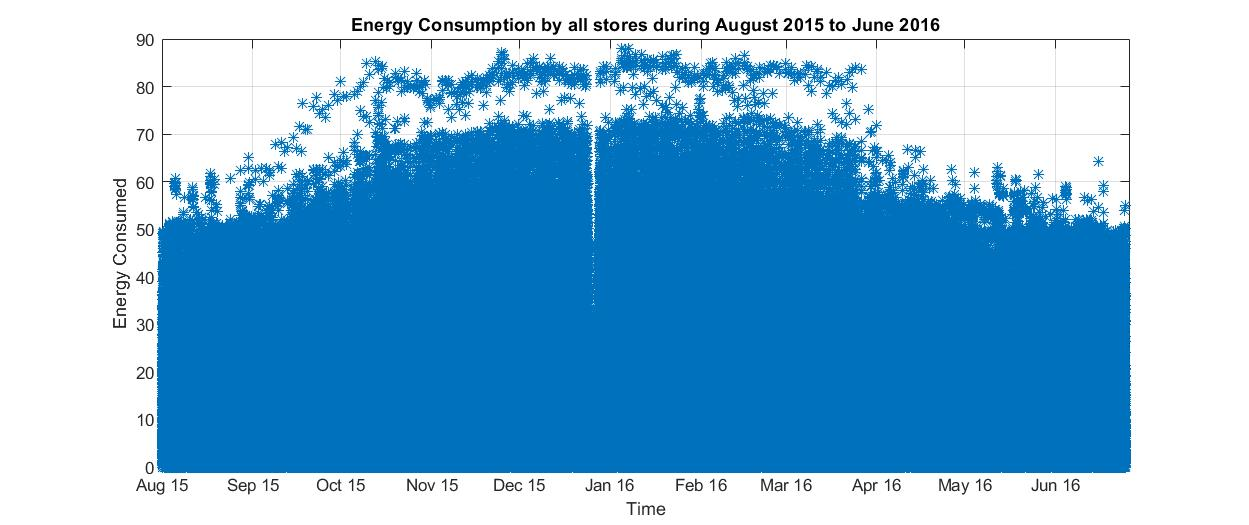
\includegraphics[width=13cm,height=5.5cm]{All_stores.jpg}
	\caption{Energy Consumption by all stores between August 2015 and June 2016}
	\label{fig:all_stores}
\end{figure*}

Afterwards, a random month is selected from the whole time period (in
this case November 2015) for visualization and energy consumption of all stores is plotted as
shown in Figure \ref{fig:all_stores_nov}.

\begin{figure*}[h]
	\centering
	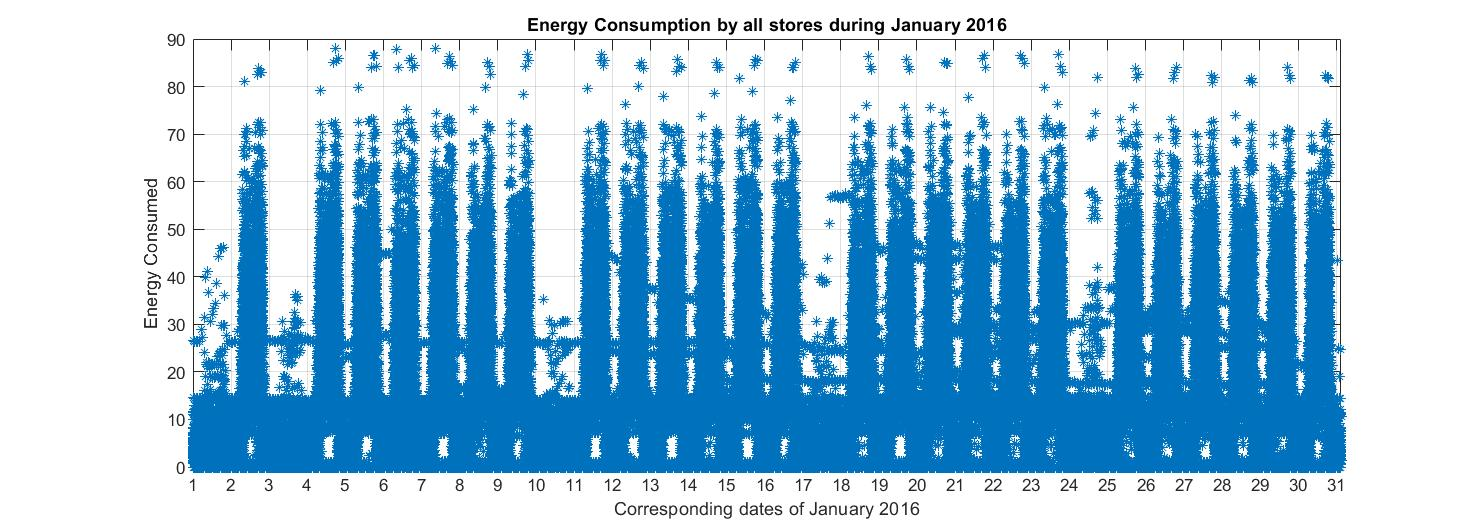
\includegraphics[width=13cm,height=5.5cm]{jan_all_stores.jpg}
	\caption{Energy Consumption by all stores during January 2016}
	\label{fig:all_stores_nov}
\end{figure*}

Still, it was difficult to pinpoint or visualize any single store from that
plot. Therefore, a random store was chosen (in this case Store 105) for in depth analysis
as shown in Figure \ref{fig:store_105_all}.

\begin{figure*}[h]
	\centering
	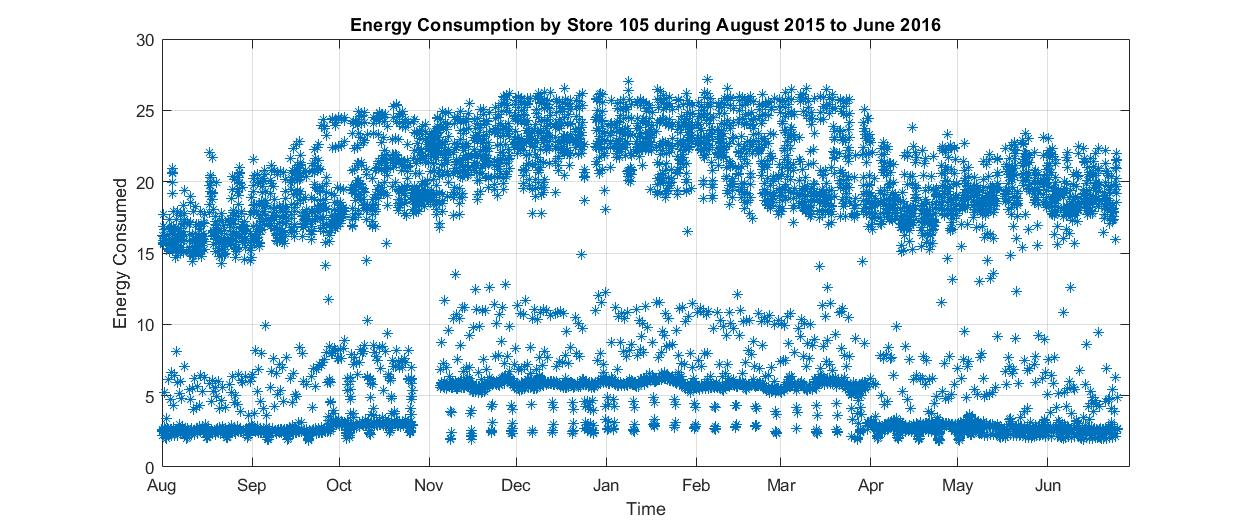
\includegraphics[width=13cm,height=5.5cm]{store_105_all.jpg}
	\caption{Energy Consumption by Store 105  between August 2015 and June 2016}
	\label{fig:store_105_all}
\end{figure*}

We can again see the noticeable increase in energy consumption during
winter months from October till April as well as lower consumption during
Christmas and New year holidays.
Again, we used November which was randomly picked earlier to visualize the
energy consumption by Store 105 as shown in Figure \ref{fig:store_105_nov}.

%\begin{figure*}[h]
%	\centering
%	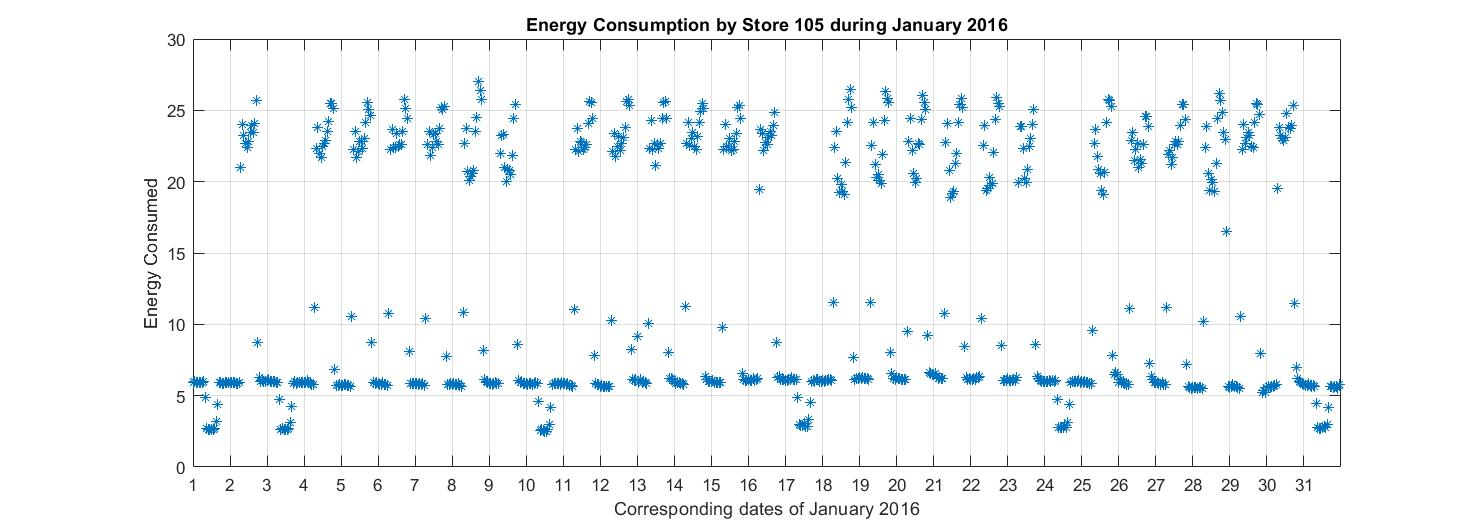
\includegraphics[width=13cm,height=5.5cm]{store_105_jan.jpg}
%	\caption{Energy Consumption by Store 105 during January 2016}
%	\label{fig:store_105_nov}
%\end{figure*}

In order to select meaningful features to be implemented in Machine Learning
or Statistical Modeling algorithms, it was necessary to analyze the given data throughly. After a comprehensive analysis, it was decided that the amount of energy
consumption depends upon multiple factors, which are the store itself as
all stores differs from one another as each having its particular size, different
number of energy consuming equipments and even have different geographical
location which affect the amount of energy consumption. Aside from that,
time of the day is another factor as during working hours energy consumption
is higher. There is also a reduction in power consumption during the day even when the store is closed.

The data consisted of the energy readings from 227 different stores with 238 sensor values (as certain stores had multiple sensors) taken every 15 minute which spanned over a period of 11 months. The provided data was then throughly examined and it was subdivided into 2 main categories which were working days and non-working days as energy consumption showed different trends in both categories. Therefore, a Feature Vector was developed which consisted of respective month, hour of the day, store number, energy consumed, a tag for working day or non-working day. As the data was gathered from the sensors in the real world therefore, it was highly unbalanced  outliers estimated to be around 2-5\% of the total dataset.

\subsection{\label{sec:level2}	Statistical Method for Outlier Detection}
In order to detect the outliers, a feature vector was developed, which consisted of the hour of the day, store number, energy consumed, a tag for working and non-working day and on that data a modified version of Tukey's test \cite{doi:10.1080/00031305.1978.10479236} was performed, which involves the calculation of median of training data which is referred to $\mathit{Q}$2 and then again median of values lesser and greater than that of $\mathit{Q}$2  is calculated. Median of values lower than $\mathit{Q}$2  is refereed as $\mathit{Q}$1  (lower quartile) and those having greater than $\mathit{Q}$2 is referred as $\mathit{Q}$3  (upper quartile) as shown in Figure 8. 

After determining $\mathit{Q}$1 and $\mathit{Q}$3, then Interquartile Range (IQR) is calculated by subtracting the value at $\mathit{Q}$3 by $\mathit{Q}$1.


After determining $\mathit{Q}$1 and $\mathit{Q}$3, then Interquartile Range (IQR) is calculated by subtracting the value at $\mathit{Q}$3 by $\mathit{Q}$1.

\begin{equation}
IQR = Q3 - Q1
\end{equation}

After calculating the IQR, we use it to calculate the Tukey's Fences or Inner Fences by the following equation,

\begin{equation}
InnerFenceLowerLimit = Q1 - \alpha (IQR)
\end{equation}
\begin{equation}
InnerFenceUpperLimit = Q1 + \alpha (IQR)
\end{equation}

where,

$\mathit{\alpha}$ is the factor which varies the inner fence limits.

\begin{figure}[t]
	\centering
	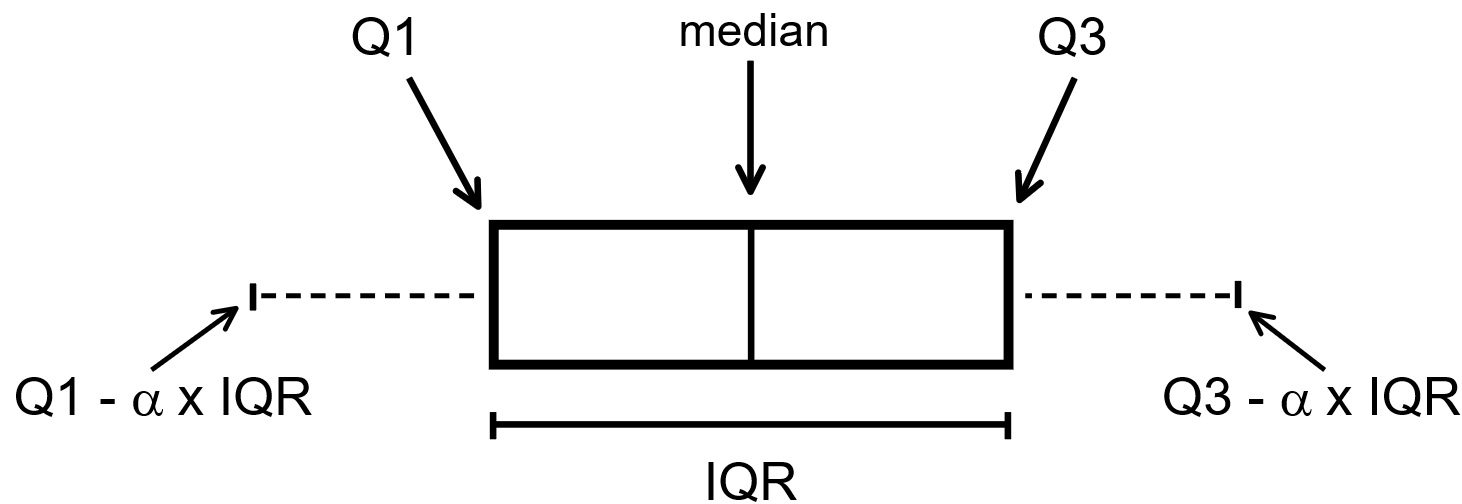
\includegraphics[width=6cm,height=2.5cm]{IQR3.jpg}
	\caption{Depiction of quartiles as used in the detection and removal of
		Outliers.}
	\label{fig:boat0}
\end{figure}

Any value lying beyond inner fence limits (upper and lower) can be considered as an 	outlier, and therefore, it is removed. The results of designed outlier detection 	algorithm are shown in Figure \ref{fig:OLX1}, \ref{fig:boat1} and \ref{fig:gull}.

As the dataset used in this project was highly varied and there were several energy values that stayed the same for the whole period of time. In order to calculate the quartiles and medians, there must be at least 4 unique values in a dataset, therefore for those dataset having less unique values, some product of their respective average was used to determine Inner and Outer Fences. 

\subsection{\label{sec:level3}	Autoencoder}

An autoencoder always consists of two parts, the encoder and the decoder, which can be defined 	as transitions $\phi$ and $\psi$ such that:

\begin{equation}
\phi : \mathcal{X} \to \mathcal{F}
\end{equation}

\begin{equation}
\psi : \mathcal{F} \to \mathcal{X}
\end{equation}

\begin{equation}
\phi , \psi = 
\argmin_{\phi,\psi}\ \| X - (\phi \circ \psi)X  \|^2\\
\end{equation}

In a simple case, if there is one hidden layer, the encoder stage of an autoencoder takes the input $\mathbf{x}$ $\in$ $\mathbb{R}^d = \mathcal{X}$ and maps it to $\mathbf{z} \in \mathbb{R}^p =\mathcal{F}  $.
\begin{equation}
\boldmath{z} = \sigma(Wx+b)
\end{equation}

This image $\mathbf {z} $  is usually referred to as \textit{code}, \textit{latent variables} or \textit{latent representation}. Here, $\sigma$ is an element-wise activation function such as sigmoid function, hyperbolic tangent or a rectified linear unit. \boldmath{W} is weight matrix and \boldmath{b} is a bias vector. After that, the decoder stage of the autoencoder maps $\mathbf{z}$ to the reconstruction $\mathbf{x^{\prime}}$ of the same shape as $\mathbf{x}$.

\begin{equation}
\boldmath{x^{\prime}} = \sigma^{\prime}(W^{\prime}z+b^{\prime})
\end{equation}

where, $\sigma^{\prime}$, $W^{\prime}$ and $b^{\prime}$ for the decoder may differ in general from the corresponding $\sigma$, $W$ and $b$ for the encoder, depending on the design of the autoencoder.

Autoencoders are also trained to minimize reconstruction errors (such as squared errors):

\begin{equation}
\mathcal{L}(x,x^{\prime}) = \|x- \sigma^{\prime}(W^{\prime}(\sigma(Wx+b))+b^{\prime})\|^2
\end{equation}

where, $x$ is usually averaged over some input training set.

If the feature space $\mathcal{F}$  has lower dimensionality than the input space $\mathcal{X}$, then the feature vector $\phi(x)$ can be regarded as a compressed representation of the input $x$.  If the hidden layers are larger than the input layer, an autoencoder can potentially learn the identity function and become useless. However, experimental results have shown that autoencoders might still learn useful features in these cases.


In case of Undercomplete autoencoders, $\mathcal{F}$ has lower dimensionality than the input space $\mathcal{X}$, then the feature vector $\phi(x)$  can be regarded as a compressed representation of the input $x$.

In this paper, an undercomplete autoencoder was trained in a semi-supervised fashion on the values of normal energy consumption data. Afterwards, the trained model was used and evaluated on a pre-trained dataset. 


\section{Experiments and Results}
\label{sec:level1}

Outlier detection algorithm was developed and it performed adequately well in removing the outliers. Figure \ref{fig:OLX} shows the energy consumption data of each hour for all working days in January 2016, where as, figure \ref{fig:OLX1} shows the
same data as in figure \ref{fig:OLX} after the outlier removal algorithm implemented on it.
\begin{figure}[h]
	%\centering
	\begin{flushleft}
			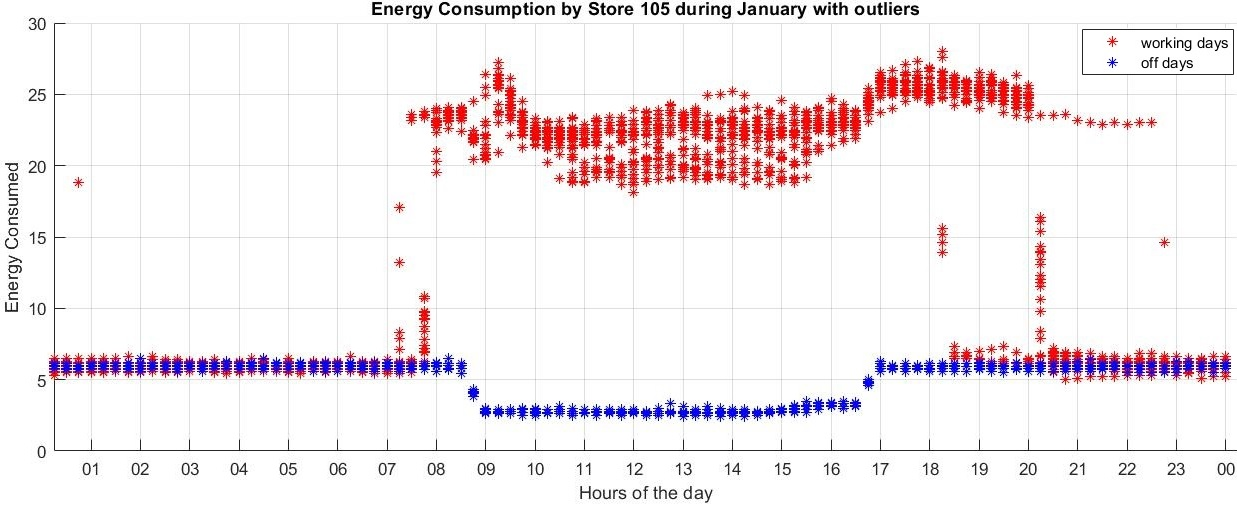
\includegraphics[width=\linewidth]{zzz.jpg}
		\caption{Energy Consumption by Store 105 during working days of January 2016 with outliers}
		\label{fig:OLX}
	\end{flushleft}

\end{figure}
\begin{figure}[h]
	%\centering
	\begin{flushleft}
	
	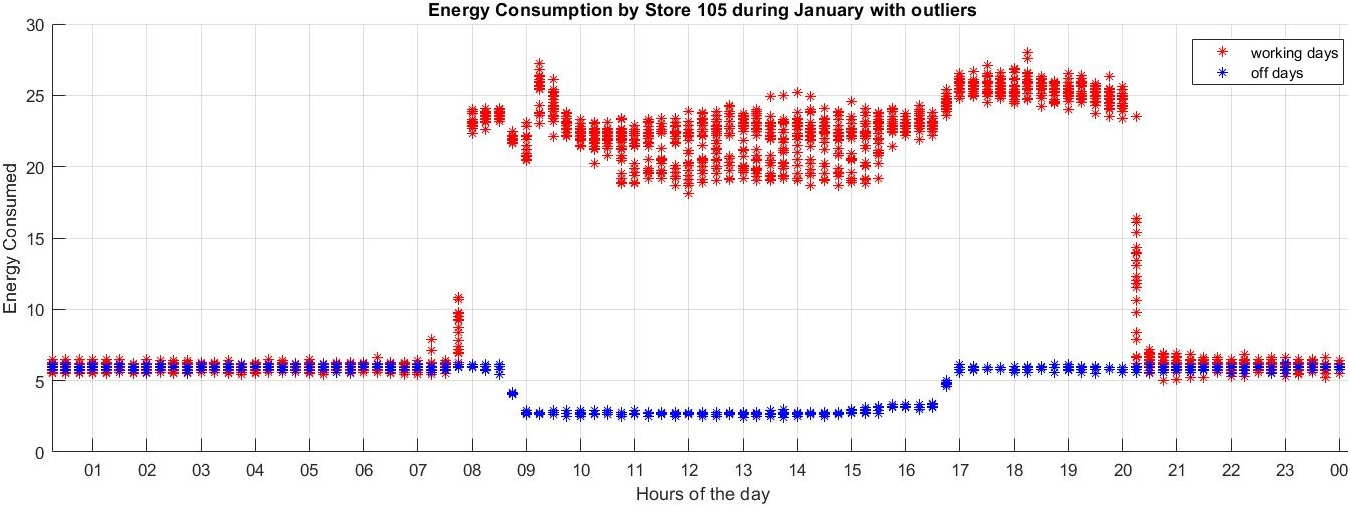
\includegraphics[width=\linewidth]{all_days_st_05_jan_wo_OL.jpg}
	\caption{Energy Consumption by Store 105 during working days of January 2016 without outliers}
	\label{fig:OLX1}
\end{flushleft}
\end{figure}

In Fig \ref{fig:conf}, we are comparing the accuracy of prediction of both algorithms with manually classified energy data of two stores using confusion matrices.

\begin{figure}[H]
	%\centering
	\subfigure[Confusion Matrix of Outlier Detection Algorithm]
	{
		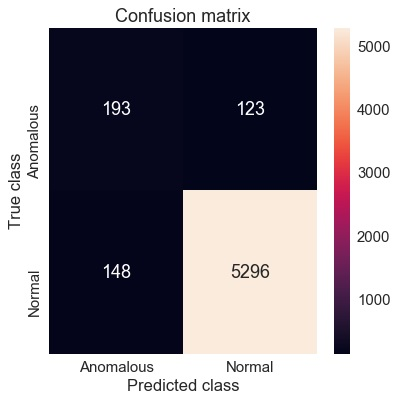
\includegraphics[width=2.5in]{conf_anomaly.jpg}
		%\caption{ROC curve of Anomaly Detection Algorithm.}
		\label{fig:boat1}
	}
	\subfigure[Confusion Matrix of Autoencoder.]
	{
		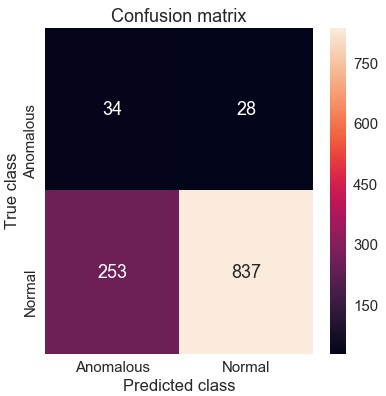
\includegraphics[width=2.5in]{Conf_autoencoder.jpg}
		\label{fig:boat2}
	}
	\caption{Confusion Matrices}
	\label{fig:conf}
\end{figure}

%\begin{figure}[]
%	%\centering
%	\begin{subfigure}{0.43\textwidth}
%		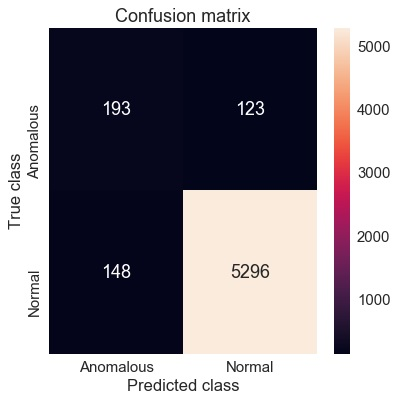
\includegraphics[width=\linewidth]{conf_anomaly.jpg}
%		\caption{Confusion Matrix of Anomaly Detection Algorithm}
%		\label{fig:boat1}
%	\end{subfigure}

%	\begin{subfigure}{0.43\textwidth}
%	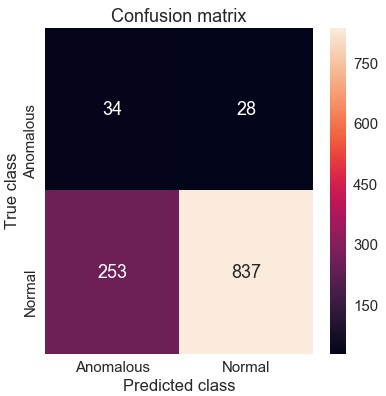
\includegraphics[width=\linewidth]{Conf_autoencoder.jpg}
%	\caption{Confusion Matrix of Autoencoder.}
%	\label{fig:boat2}
%\end{subfigure}
%\caption{Confusion Matrices}
%\label{fig:conf}
%\end{figure}



%\begin{figure}[h]
%	\centering
%	\begin{subfigure}{0.45\textwidth}
%		\includegraphics[width=\textwidth]{roc_anomaly.jpg}
%		\caption{ROC curve of Anomaly Detection Algorithm.}
%		\label{fig:gull}
%	\end{subfigure}
~ %add desired spacing between images, e. g. ~, \quad, \qquad, \hfill etc. 
%(or a blank line to force the subfigure onto a new line)
%	\begin{subfigure}{0.45\textwidth}
%		\includegraphics[width=\textwidth]{roc_autoencoder.jpg}
%		\caption{ROC curve of Autoencoder.}
%		\label{fig:tiger}
%	\end{subfigure}
%	\caption{ROC curves}
%	\label{fig:ROC}

%\end{figure}
The same dataset which was used to make confusion matrices in Fig \ref{fig:conf} is used to plot Receiver Operating Characteristics curves in Fig \ref{fig:ROC}.
\begin{figure}[H]
	%\centering
	\subfigure[ROC curve of Outlier Detection Algorithm.]
	{
		\includegraphics[width=2.5in]{roc_anomaly.jpg}
		
		\label{fig:gull}
	}
	\subfigure[ROC curve of Autoencoder.]
	{
		\includegraphics[width=2.5in]{roc_autoencoder.jpg}
		\label{fig:tiger}
	}
	\caption{ROC curves}
	\label{fig:ROC}
	
\end{figure}




 


The same dataset which was used to make confusion matrices in Fig \ref{fig:conf} is used to plot Receiver Operating Characteristics curves in Fig \ref{fig:ROC}.




As we can see from the comparison of Fig \ref{fig:conf} and Fig \ref{fig:ROC}, we can interpret that the performance of Statistical method which is based on Tukey's test performed remarkably better with around 95\% correlation with manual classification but the shortcoming of this method is that the dataset should be arranged in a proper manner as a single missing values in the dataset can make the classification ineffective. Whereas, classification using Autoencoder performed adequately with around 70-75\% correlation with manually classified data but it required pre-classified data containing no outliers.  

\section{Discussion/Outlook/Conclusion/Future Work}

In this paper, the performance of a semi supervised Autoencoder and a statistical model for outlier detection was compared. The experiment resulted in the varying results from each algorithms as Autoencoder did not require data to be arranged precisely and were robust against mixed up dataset whereas, Statistical based outlier detection model performed more accurately in detecting outliers but it required careful arrangement of the data.


In future, it is planned to use more variables in the feature vector of energy consumption data such size of the facility, number of energy consuming equipments, occupancy of the building, and other sensor data such as outside temperature and solar radiation. As more data is embedded in the feature vector, there will be more focus on using totally unsupervised learning using Autoencoder to discover and learn new pattern in the given dataset and do the classification more precisely.

%\section{MMSN Protocol}

% Head 2
%\subsection{Frequency Assignment}

%We propose a suboptimal distribution to be used by each node, which is
%easy to compute and does not depend on the number of competing
%nodes. A natural candidate is an increasing geometric sequence, in
%which
% Numbered Equation
%\begin{equation}
%\label{eqn:01}
%P(t)=\frac{b^{\frac{t+1}{T+1}}-b^{\frac{t}{T+1}}}{b-1},
%\end{equation}
%where $t=0,{\ldots}\,,T$, and $b$ is a number greater than $1$.

%In our algorithm, we use the suboptimal approach for simplicity and
%generality. We need to make the distribution of the selected back-off
%time slice at each node conform to what is shown in Equation
%(\ref{eqn:01}). It is implemented as follows: First, a random
%variable $\alpha$ with a uniform distribution within the interval
%$(0, 1)$ is generated on each node, then time slice $i$ is selected
%according to the following equation:
% Unnumbered Equation
%\[
%i=\lfloor(T+1)\log_b[\alpha(b-1)+1]\rfloor.
%\]
%It can be easily proven that the distribution of $i$ conforms to Equation
%(\ref{eqn:01}).

%So protocols [Bahl 2002,Culler 2001,Zhou 2006,Adya 2001,Culler 2001;
%Tzamaloukas-01; Akyildiz-01] that use RTS/CTS
%controls\footnote{RTS/CTS controls are required to be implemented by
%802.11-compliant devices. They can be used as an optional mechanism
%to avoid Hidden Terminal Problems in the 802.11 standard and
%protocols based on those similar to [Akyildiz 2001] and
%[Adya 2001].} for frequency negotiation and reservation are not
%suitable for WSN applications, even though they exhibit good
%performance in general wireless ad hoc
%networks.

% Head 3
%\subsubsection{Exclusive Frequency Assignment}

%In exclusive frequency assignment, nodes first exchange their IDs
%among two communication hops so that each node knows its two-hop
%neighbors' IDs. In the second broadcast, each node beacons all
%neighbors' IDs it has collected during the first broadcast period.

% Head 4
%\paragraph{Eavesdropping}

%Even though the even selection scheme leads to even sharing of
%available frequencies among any two-hop neighborhood, it involves a
%number of two-hop broadcasts. To reduce the communication cost, we
%propose a lightweight eavesdropping scheme.

%\subsection{Basic Notations}

%As Algorithm~\ref{alg:one} states, for each frequency
%number, each node calculates a random number (${\textit{Rnd}}_{\alpha}$) for
%itself and a random number (${\textit{Rnd}}_{\beta}$) for each of its two-hop
%neighbors with the same pseudorandom number generator.
% Algorithm
%\begin{algorithm}[t]
%\SetAlgoNoLine
%\KwIn{Node $\alpha$'s ID ($ID_{\alpha}$), and node $\alpha$'s
%neighbors' IDs within two communication hops.}
%\KwOut{The frequency number ($FreNum_{\alpha}$) node $\alpha$ gets assigned.}
%$index$ = 0; $FreNum_{\alpha}$ = -1\;
%\Repeat{$FreNum_{\alpha} > -1$}{
%        $Rnd_{\alpha}$ = Random($ID_{\alpha}$, $index$)\;
%        $Found$ = $TRUE$\;
%        \For{each node $\beta$ in $\alpha$'s two communication hops
%    }{
%      $Rnd_{\beta}$ = Random($ID_{\beta}$, $index$)\;
%      \If{($Rnd_{\alpha} < Rnd_{\beta}$) \text{or} ($Rnd_{\alpha}$ ==
%          $Rnd_{\beta}$ \text{and} $ID_{\alpha} < ID_{\beta}$)\;
%      }{
%        $Found$ = $FALSE$; break\;
%      }
%        }
%     \eIf{$Found$}{
%           $FreNum_{\alpha}$ = $index$\;
%         }{
%           $index$ ++\;
%     }
%      }
%\caption{Frequency Number Computation}
%\label{alg:one}
%\end{algorithm}

%Bus masters are divided into two disjoint sets, $\mathcal{M}_{RT}$
%and $\mathcal{M}_{NRT}$.
% description
%\begin{description}
%\item[RT Masters]
%$\mathcal{M}_{RT}=\{ \vec{m}_{1},\dots,\vec{m}_{n}\}$ denotes the
%$n$ RT masters issuing real-time constrained requests. To model the
%current request issued by an $\vec{m}_{i}$ in $\mathcal{M}_{RT}$,
%three parameters---the recurrence time $(r_i)$, the service cycle
%$(c_i)$, and the relative deadline $(d_i)$---are used, with their
%relationships.
%\item[NRT Masters]
%$\mathcal{M}_{NRT}=\{ \vec{m}_{n+1},\dots,\vec{m}_{n+m}\}$ is a set
%of $m$ masters issuing nonreal-time constrained requests. In our
%model, each $\vec{m}_{j}$ in $\mathcal{M}_{NRT}$ needs only one
%parameter, the service cycle, to model the current request it
%issues.
%\end{description}

%Here, a question may arise, since each node has a global ID. Why
%don't we just map nodes' IDs within two hops into a group of
%frequency numbers and assign those numbers to all nodes within two
%hops?









% Start of "Sample References" section

%\section{Typical references in new ACM Reference Format}
%A paginated journal article \cite{Abril07}, an enumerated journal article \cite{Cohen07}, a reference to an entire issue \cite{JCohen96},
%a monograph (whole book) \cite{Kosiur01}, a monograph/whole book in a series (see 2a in spec. document)
%\cite{Harel79}, a divisible-book such as an anthology or compilation \cite{Editor00}
%followed by the same example, however we only output the series if the volume number is given
%\cite{Editor00a} (so Editor00a's series should NOT be present since it has no vol. no.),
%a chapter in a divisible book \cite{Spector90}, a chapter in a divisible book
%in a series \cite{Douglass98}, a multi-volume work as book \cite{Knuth97},
%an article in a proceedings (of a conference, symposium, workshop for example)
%(paginated proceedings article) \cite{Andler79}, a proceedings article
%with all possible elements \cite{Smith10}, an example of an enumerated
%proceedings article \cite{VanGundy07},
%an informally published work \cite{Harel78}, a doctoral dissertation \cite{Clarkson85},
%a master's thesis: \cite{anisi03}, an online document / world wide web resource \cite{Thornburg01}, \cite{Ablamowicz07},
%\cite{Poker06}, a video game (Case 1) \cite{Obama08} and (Case 2) \cite{Novak03}
%and \cite{Lee05} and (Case 3) a patent \cite{JoeScientist001},
%work accepted for publication \cite{rous08}, 'YYYYb'-test for prolific author
%\cite{SaeediMEJ10} and \cite{SaeediJETC10}. Other cites might contain
%'duplicate' DOI and URLs (some SIAM articles) \cite{Kirschmer:2010:AEI:1958016.1958018}.
%Boris / Barbara Beeton: multi-volume works as books
%\cite{MR781536} and \cite{MR781537}.

% Appendix
%\appendix
%\section*{APPENDIX}
%\setcounter{section}{1}
%In this appendix, we measure
%the channel switching time of Micaz [CROSSBOW] sensor devices.
%In our experiments, one mote alternatingly switches between Channels
%11 and 12. Every time after the node switches to a channel, it sends
%out a packet immediately and then changes to a new channel as soon
%as the transmission is finished. We measure the
%number of packets the test mote can send in 10 seconds, denoted as
%$N_{1}$. In contrast, we also measure the same value of the test
%mote without switching channels, denoted as $N_{2}$. We calculate
%the channel-switching time $s$ as
%\begin{eqnarray}%
%s=\frac{10}{N_{1}}-\frac{10}{N_{2}}. \nonumber
%\end{eqnarray}%
%By repeating the experiments 100 times, we get the average
%channel-switching time of Micaz motes: 24.3$\mu$s.

%\appendixhead{ZHOU}

% Acknowledgments
%\begin{acks}
%Italia for providing specifications about the %application scenario.
%\end{acks}

% Bibliography
\bibliographystyle{ACM-Reference-Format-Journals}
\bibliography{acmsmall-sample-bibfile}
                             % Sample .bib file with references that match those in
                             % the 'Specifications Document (V1.5)' as well containing
                             % 'legacy' bibs and bibs with 'alternate codings'.
                             % Gerry Murray - March 2012

% History dates
%\received{February 2007}{March 2009}{June 2009}

% Electronic Appendix
%\elecappendix

%\medskip

%\section{This is an example of Appendix section head}

%Channel-switching time is measured as the time length it takes for
%motes to successfully switch from one channel to another. This
%parameter impacts the maximum network throughput, because motes
%cannot receive or send any packet during this period of time, and it
%also affects the efficiency of toggle snooping in MMSN, where motes
%need to sense through channels rapidly.

%By repeating experiments 100 times, we get the average
%channel-switching time of Micaz motes: 24.3 $\mu$s. We then conduct
%the same experiments with different Micaz motes, as well as
%experiments with the transmitter switching from Channel 11 to other
%channels. In both scenarios, the channel-switching time does not have
%obvious changes. (In our experiments, all values are in the range of
%23.6 $\mu$s to 24.9 $\mu$s.)

%\section{Appendix section head}

%The primary consumer of energy in WSNs is idle listening. The key to
%reduce idle listening is executing low duty-cycle on nodes. Two
%primary approaches are considered in controlling duty-cycles in the
%MAC layer.

\end{document}
% End of v2-acmsmall-sample.tex (March 2012) - Gerry Murray, ACM


